% Intended LaTeX compiler: pdflatex
\documentclass[bigger]{beamer}
\usepackage[utf8]{inputenc}
\usepackage[T1]{fontenc}
\usepackage{graphicx}
\usepackage{longtable}
\usepackage{wrapfig}
\usepackage{rotating}
\usepackage[normalem]{ulem}
\usepackage{amsmath}
\usepackage{amssymb}
\usepackage{capt-of}
\usepackage{hyperref}
\mode<beamer>{\usetheme{Madrid}}
\mode<beamer>{\usepackage{amsmath}}
\usetheme{default}
\author{Konstantinos Papadimos}
\date{}
\title{Presentation draft}
\hypersetup{
 pdfauthor={Konstantinos Papadimos},
 pdftitle={Presentation draft},
 pdfkeywords={},
 pdfsubject={},
 pdfcreator={Emacs 28.2 (Org mode 9.5.5)}, 
 pdflang={English}}
\begin{document}

\maketitle

\section{Introductory stuff, Detectros and Particle physics}
\label{sec:org9804ab0}
\begin{frame}[label={sec:org38a8f7c}]{The CMS Experiment overview}
The CMS detector at the LHC
\begin{figure}[hb]
\centering
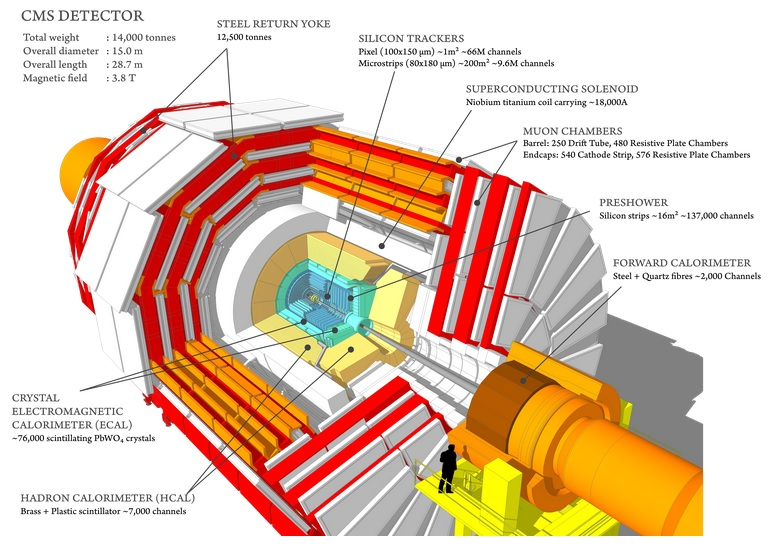
\includegraphics[width=0.7 \textwidth, ext=.png type=jpg]{/home/kpapad/UG_thesis/Thesis/Dissertation/src/figures/cms_detector.jpg}
\end{figure}
\end{frame}

\begin{frame}[label={sec:org87e6f81}]{Coordinates at the CMS}
Given the solenoid geometry of the CMS detector, it is more convenient to use a spherical type of coordinates\(\left(r, \phi, \theta \right)\).
\begin{equation}
\begin{matrix}
p_{x} = P_{T}\cos{\phi} \\
p_{y} = P_{T}\sin{\phi} \\
p_{z} = P_{T}\sinh{\eta}\\
|\vec{P}| = P_{T}\cosh{\eta} 
\end{matrix}
\end{equation}
\(\phi \in \left [ 0, 2\pi \right]\)the azimuthal angle, and \(\eta\in \left [ -\infty, +\infty \right ]\) is defined as:
\begin{equation}
\eta \equiv -\ln{\left [ \tan\left (\frac{\theta}{2} \right ) \right]  }
\end{equation}
\end{frame}

\begin{frame}[label={sec:orga42626a}]{Decays \& Resonances}
Not every particle can be detected by the CMS detector(i.e neutrinos)
\begin{columns}
\begin{column}{0.5\columnwidth}
\begin{itemize}
\item Detectable Decay Products \(\rightarrow\) Resonance
\end{itemize}
\begin{center}
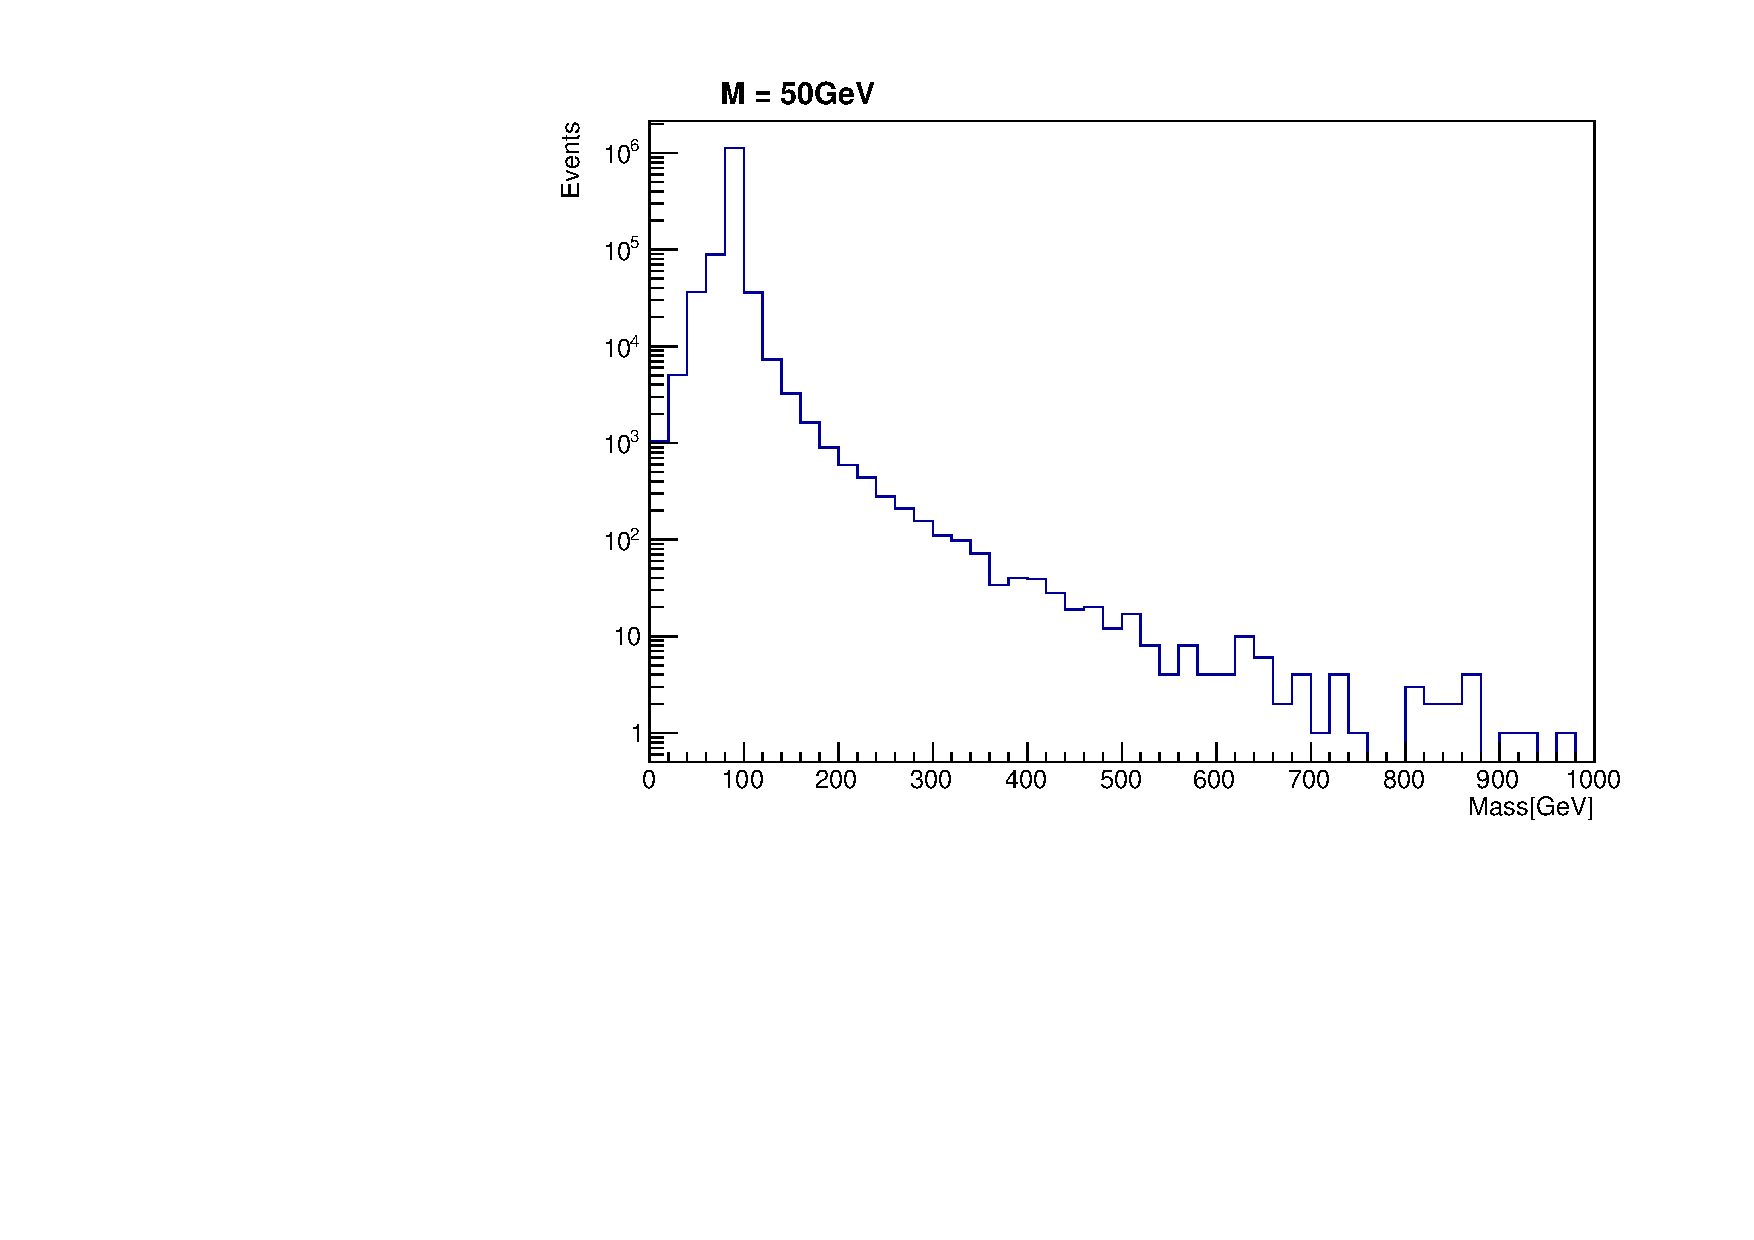
\includegraphics[width=0.8\textwidth]{/home/kpapad/UG_thesis/Thesis/Analysis/out/Plots/DYJetsM50_MassHist.pdf}
\end{center}
\end{column}

\begin{column}{0.5\columnwidth}
\begin{itemize}
\item Non Detectable Decay Products \(\rightarrow\) Not a resonance
\end{itemize}
\begin{center}
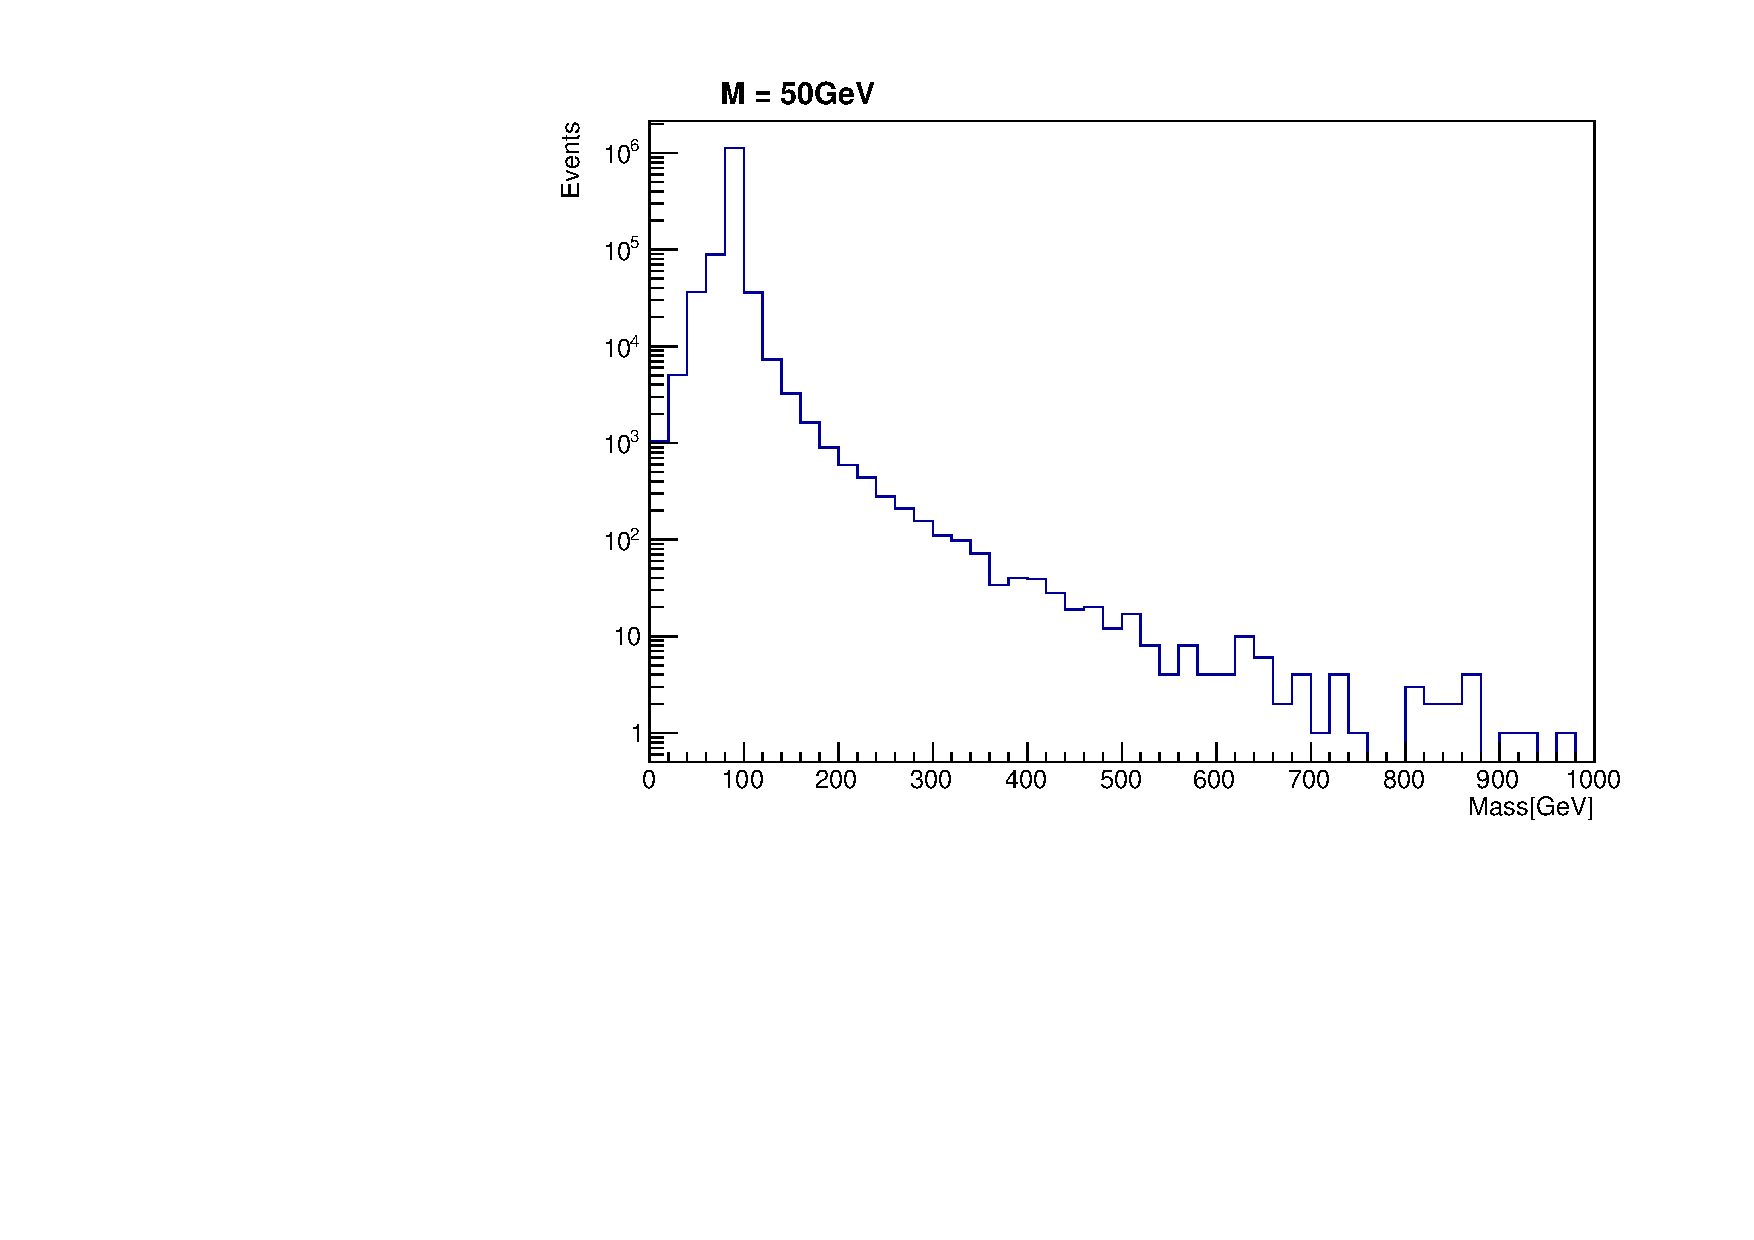
\includegraphics[width=.9\linewidth]{/home/kpapad/UG_thesis/Thesis/Analysis/out/Plots/DYJetsM50_MassHist.pdf}
\end{center}
\end{column}
\end{columns}
\end{frame}

\begin{frame}[label={sec:org2d3dc06}]{Callibration and energy scale uncertainties}
\begin{itemize}
\item Calibration process adjusts energy scale and resolution to match well-known resonances (Z boson, J/psi meson) in data and simulation,
\end{itemize}
\begin{itemize}
\item Imperfect agreement due to subdetector complexities and nonlinear effects
\end{itemize}
\begin{block}{How do analysis techniques respond to energy scale uncertainties ?}
Our work will focus on the effects that energy scale uncertainties have, in a traditional fit-based analysis and a more modern Boosted Decision Tree-based analysis, using the generic diobject production process as the working example.
\end{block}
\end{frame}
\section{Analysis techniqies}
\label{sec:org44745d0}
\begin{frame}[label={sec:orge39b4fa}]{BDT 1}
Explain what a bdt is. There is a nice example in XGBoost documentation. 
\end{frame}
\begin{frame}[label={sec:orgc2a4e94}]{BDT 2}
Explain the train->test->Application workflow. 
\end{frame}
\begin{frame}[label={sec:orgd69b9ae}]{BDT 3}
Talk about the output, explain what the BDT score is and what BDT histogram is. Discuss signal from backgroun separation using bdt
\end{frame}
\begin{frame}[label={sec:org597d79b}]{Fit}
Explain fit based signal from backgroun separation
\end{frame}
\begin{frame}[label={sec:org2203ef3}]{Statistical interpretation of results}
Talk about significance.
\end{frame}
\section{Analysis}
\label{sec:orgfbec8f3}
\begin{frame}[label={sec:org777bb3b}]{Energy scale uncertainties}
How we implemented the smearing in our data set. How do we proceed from that, how many smearing cases. 
\end{frame}
\begin{frame}[label={sec:orgb59b6e5}]{BDT approach 1}
Train Testing application set. Summarize the number of events. Explain that in order to compare apples to apples, we will be analyzing the application set from now on.
\end{frame}
\begin{frame}[label={sec:org89e91c5}]{BDT approach 2}
Application summarize the results 
\end{frame}
\begin{frame}[label={sec:org7e4723b}]{Fit based approach 1}
Show the mass spectrum that will be fitted 
\end{frame}
\begin{frame}[label={sec:orga2ddd25}]{Fit based approach 2}
discuss bkg fit is kept constnat throughout the analysis. discus signal fitting, show the plots( I will probably need more than one slide) at this part talk about the fact that after \(20\%\) the fit based technique fails. 
\end{frame}
\begin{frame}[label={sec:orgb41d5fc}]{Fit based approach 2}
Present the significances.
\end{frame}
\section{Results}
\label{sec:org96406ef}
\begin{frame}[label={sec:org58764e7}]{Results 1}
Compare the BDT and FIt in terms of significance and robustness. Comment that even though fit based achieves a higher significance in the 0 smearing case, it is not as robust as bdt, it completelly fails at extreme cases of smearing,. BDT is more robust 
\end{frame}
\begin{frame}[label={sec:org8e67c7d}]{Results 2}
Try to explain that bdt uses not only energy related features (Pts) but also geometrical ones, which do not get affected by smearing. Therefore, more stabillity to smearing. Nevertheless robustness does not mean greateer classification "power"(how many events got classified correctly and how manny didn't) -->Outlooks for better training methods in other to increase classification power.   
\end{frame}
\section{Unused stuff}
\label{sec:orga7db2b1}
\begin{frame}[label={sec:org1d43604}]{Resonance text}
and therefore, the invariant mass calculation from the detected particles of such events will not result in a peak at the mass spectrum(Non resonant proces). Even though in decays where  the poducts are detectable particles, the invariant mass calculation leads to a peak in the mass spectrum(resonant decays). In the present work we are interested in the later.
\end{frame}
\end{document}